\section{Graukonvertierung: Farbbild nach Graubild}
\label{Graubild}
Da die Berechnungen von ElSe auf Graubildern arbeitet und das Eingabebild in Farbe ist, muss es in ein Graubild umgewandelt werden.\\
Die Wahl des Verfahrens beruht auf der Anforderung, dass vor allem der Farbunterschied zwischen Pupille und der Umgebung maximal sein soll, die Pupille möglichst dunkel und das restliche Auge hell. Die Farbe der Iris erschwert die Differenzierung zusätzlich, wenn diese recht dunkel ausfällt ist auch der Unterschied zur Pupille entsprechend gering in den Grauwerten. Außerdem ist das Erkennen der Pupille bei sehr kleinen Bildern schwierig bis unmöglich wodurch auf der Iris gerechnet werden muss, und daher diese weiterhin erhalten bleiben sollte.\\
Nach der Umwandlung wird für die Anwendung das Graubild noch normiert, damit mindestens ein schwarzes und ein weißes Pixel vorhanden ist.\\
Die Auswahl von Gleam basiert auf den Ergebnissen von \glqq Color-to-Grayscale: Does the Method Matter in Image Recognition?\grqq \cite{rgb_to_Gray} und New-Gleam als eine Umsetzung des dort veröffentlichtem Ausblicks. Luminance als Standart , Quadrat als gegenstück zu Gleam und Min/Max aus der Idee der farbigen Iris.\\
Das Eingabebild der Beispiele zu den einzelnen Graukonvertierung ist in \autoref{img_Gray_Einagbe} dargestellt. Eine Farbpalette, das Bildverarbeitungsbeispiel Lena sowie ein Augenbereich aus dem Augendatensatz \cite{database_Eye}. 
\begin{figure}
	\centering
	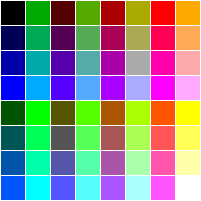
\includegraphics[width=0.2\linewidth]{img/Farbtafel2}
	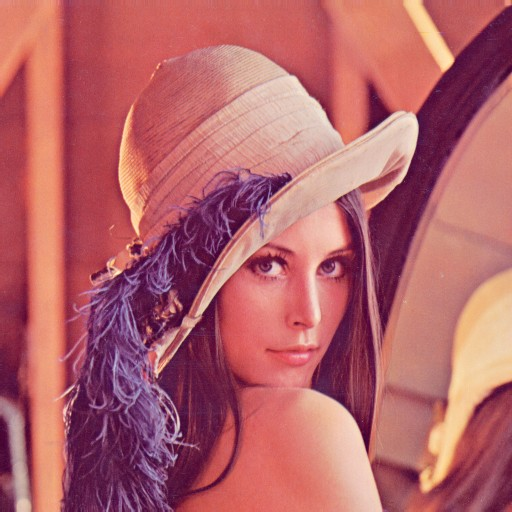
\includegraphics[width=0.2\linewidth]{img/lena}
	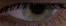
\includegraphics[width=0.2\linewidth]{img/Auge}
	\caption{Dies sind die Eingabebilder der verschiedenen Konverter von Farbe nach Grau. Links eine Farbpalette, Mitte Lena und Rechts ein Augenausschnitt aus dem Augendatensatz \cite{database_Eye}}
	\label{img_Gray_Einagbe}
\end{figure}
\subsection{Gleam-Verfahren}
\label{gray_Gleam}
Bei dem Gleam-Verfahren wird jede Farbe (Rot,Gelb und Grün) gleich stark bewertet allerdings wird jeder Farbwert mittels einer Gamma-Korrektur verändert und das Bild wirkt heller als bei dem Luminance-Verfahren.\\
Durch die Gamma-Korrektur wird vor allem der helle Bereich weiter erhöht, somit wird der Farbunterschied zwischen Iris und Auge vermindert, wodurch die Pupille der einzige dunkle Bereich wird.\\
Allerdings wird auch dieser Farbwert erhöht und sollte die Pupille nicht schwarz sein, wird sie eher ins Graue überführt, siehe \autoref{img_Gleam}.\\
\[G_{Gleam}=\dfrac{R^{\frac{1}{2.2}} + G^{\frac{1}{2.2}} + B^{\frac{1}{2.2}}}{3}\]
\subsection{Gleam-New-Verfahren}
\label{gray_New}
Dies ist eine Variante von Gleam bei dem zuerst das gesamte Bild analysiert wird um die Parameter für die jeweilige Gamma-Korrektur zu ermitteln. Dies ist etwas aufwendiger, aber für die kleinen Bilder hinnehmbar.\\
Durch die individuelle Veränderung der Farbkanäle, werden Farbunterschiede minimiert und somit alle stark farbigen Bereiche ebenfalls dunkel dargestellt. Der Kontrast zwischen der farbigen Iris und dem weißen Auge wird verbessert, siehe \autoref{img_NewGeam}.\\
Da allerdings alle Farben dunkel werden, entstehen weitere dunkle Bereiche die die Detektion der Pupille beeinträchtigen können.
\[G_{Gleam New}=\dfrac{R^{r} + G^{g} + B^{b}}{3}\]
Wobei gilt $\{r,g,b\} = \frac{\log(V_{\max})}{\log(\{R,G,B\}_{\max})}$ mit $V_{\max}$ als maximal möglicher Farbwert und $R_{\max}$ als maximal Vorhandener Rot-Wert, $G_{\max}$ und $B_{\max}$ äquivalent.
\subsection{Luminance-Verfahren}
\label{gray_Luminance}
Dies ist ein lineares Verfahren, das der menschlichen Farbwahrnehmung entspricht und oft den Standard bei der Umwandlung von Farbbild nach Graubild darstellt. Somit entsteht ein natürlicher Farbverlauf, bei dem der Farbunterschied zwischen Pupille, Iris und Auge auf einem mittleren Niveau bleibt, siehe \autoref{img_Luminance}.\\
Eine Gamma-Korrektur wird bei der Umwandlung nicht verwendet.
\[G_{Luminance} = 0.299 \cdot R + 0.587 \cdot G + 0.114 \cdot B\]
\subsection{Min-Max-Verfahren}
\label{gray_MinMax}
Dabei handelt es sich eigentlich um zwei verschiedene Varianten, allerdings funktionieren beide nach dem selben Prinzip. Als Grauwert wird der jeweilige Extremwert aus den einzelnen Farbkanälen des Pixels gewählt.\\
Durch Verwendung der Extremwerte, ist nur noch der Wert von Relevanz, nicht die eigentliche Farbe, wodurch das gesamte Bild deutlich heller bzw. dunkler wird.\\
Bei dem Max-Verfahren werden alle farbigen und helle Bereiche hell dargestellt und nur gleichmäßig dunkel Bereiche bleiben dunkel wie es bei schwarz der Fall ist. Wenn der Minimalwert anstelle verwendet wird, bleiben nur gleichmäßig helle Bereiche hell, alle anderen werden abgedunkelt.
\begin{align*}
G_{Max} &= \max(R,G,B)\\
G_{Min} &= \min(R,G,B)
\end{align*}
\subsection{Quadrat-Verfahren}
\label{gray_Quadrat}
Dies ist ein Verfahren, dass das Eingabebild verdunkelt und vom Aufbau dem Inversen von Gleam entspricht. Somit ist das gesamte Bild dunkler als bei dem Luminance-Verfahren, siehe \autoref{img_Quadrat}.\\
Durch die Abdunklung werden kleine Farbänderungen in den dunklen Bereichen reduziert, wodurch die Pupille sehr dunkel und der Farbunterschied zur Iris geringer ausfällt.
\[G_{Quadrat}=\dfrac{R^2+G^2+B^2}{3}\]
\subsection{Normalisierung der Graubilder}
Um ein Graubild zu erhalten, das das volle Spektrum der möglichen Grauwerte erfüllt, wird das Eingabebild normalisiert. Dazu wird der Maximale $G_{max}$ und Minimale $G_{min}$ Grauwert im Bild gesucht. Anschließend wird der neue Grau-Wert $G_{new}$ wie folgt bestimmt:
\[G_{new} = (G-G_{min})\cdot \dfrac{V_{max}}{G_{max}-G_{min}}\]
Dabei ist $V_{max}$ der maximale mögliche Wert in der Ausgabe und $G$ der aktuelle Grauwert im Bild.\\
Da für die Anwendung ein schwarzer Bereich gegen einen hellen Hintergrund gesucht wird, wird für die Bestimmung der Extremwerte nicht das originale Bild verwendet, sonder ein Gauß-gefiltertes.\\
Dies hat den Vorteil, dass einzelne lokal auftretende Werte, z.B. Reflektionen, nicht als Extremwert verwendet werden, wodurch die Pupille gleichmäßiger dunkler und das gesamte Bild stärker aufgehellt wird.
\subsubsection{Auswirkung des Gauß-Filters}
Dies ist ein Tiefpassfilter und wird verwendet um das Eingangssignal zu glätten. Dies hat in der Bildverarbeitung den Effekt, dass Details im Bild verschwimmen und das Bild unscharf wird.\\
Die einzelnen Werte werden ihrer Umgebung angepasst, wodurch lokal auftretende Extremar verschwinden bzw. abgeschwächt werden und ähnliche Farbwerte zu ihrer Umgebung erhalten bleiben.
\begin{figure}
	\centering
	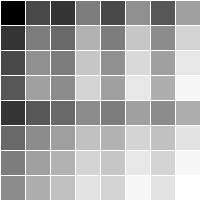
\includegraphics[width=0.21\linewidth]{img/Farbkarte2}
	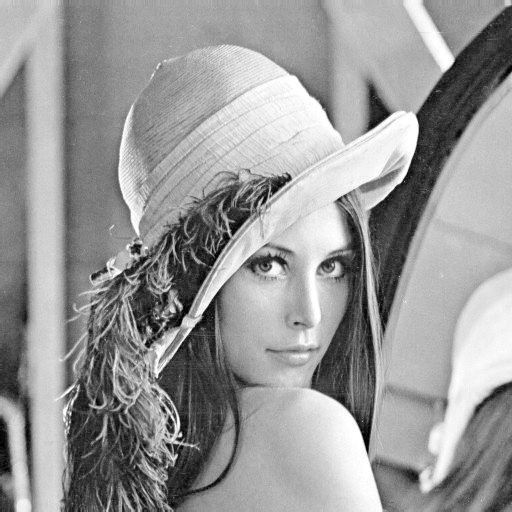
\includegraphics[width=0.21\linewidth]{img/Lena2}
	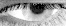
\includegraphics[width=0.21\linewidth]{img/Auge_2Gray}
	\caption{Ergebnis der Umwandlung von Farb- nach Grauwert mittels Gleam-Verfahren}
	\label{img_Gleam}
\end{figure}
\begin{figure}
	\centering
	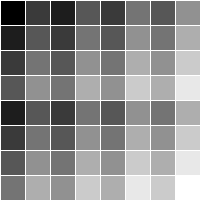
\includegraphics[width=0.21\linewidth]{img/Farbkarte1}
	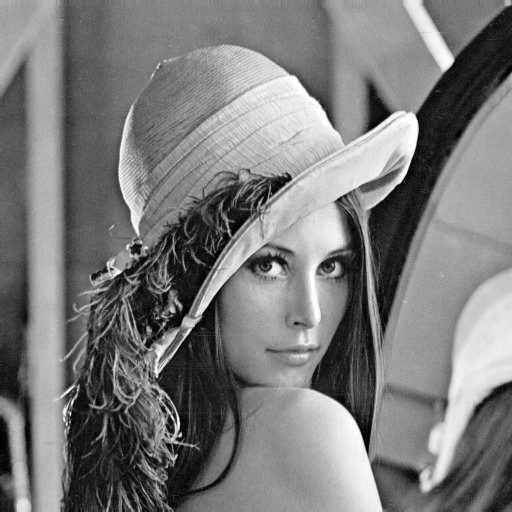
\includegraphics[width=0.21\linewidth]{img/Lena1}
	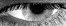
\includegraphics[width=0.21\linewidth]{img/Auge_1Gray}
	\caption{Ergebnis der Umwandlung von Farb- nach Grauwert mittels Gleam-New-Verfahren}
	\label{img_NewGeam}
\end{figure}
\begin{figure}
	\centering
	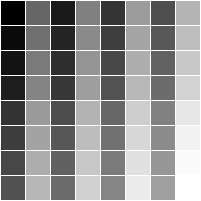
\includegraphics[width=0.21\linewidth]{img/Farbkarte0}
	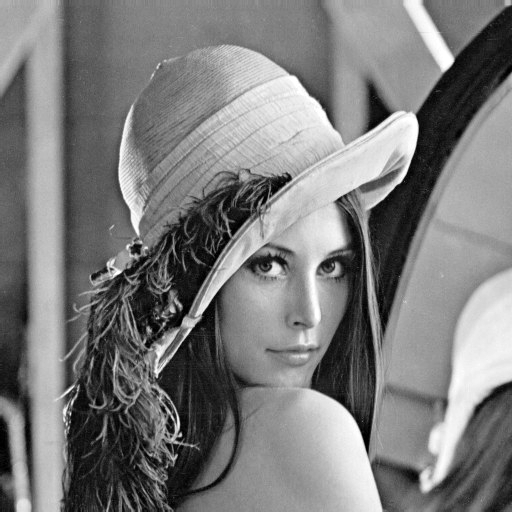
\includegraphics[width=0.21\linewidth]{img/Lena0}
	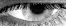
\includegraphics[width=0.21\linewidth]{img/Auge_0Gray}
	\caption{Ergebnis der Umwandlung von Farb- nach Grauwert mittels Luminance-Verfahren}
	\label{img_Luminance}
\end{figure}
\begin{figure}
	\centering
	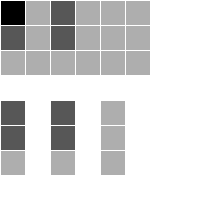
\includegraphics[width=0.21\linewidth]{img/Farbkarte5}
	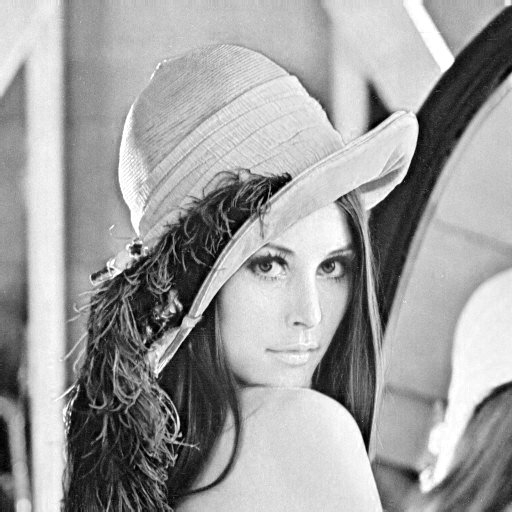
\includegraphics[width=0.21\linewidth]{img/Lena5}
	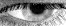
\includegraphics[width=0.21\linewidth]{img/Auge_5Gray}\\
	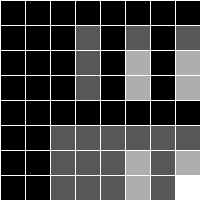
\includegraphics[width=0.21\linewidth]{img/Farbkarte4}
	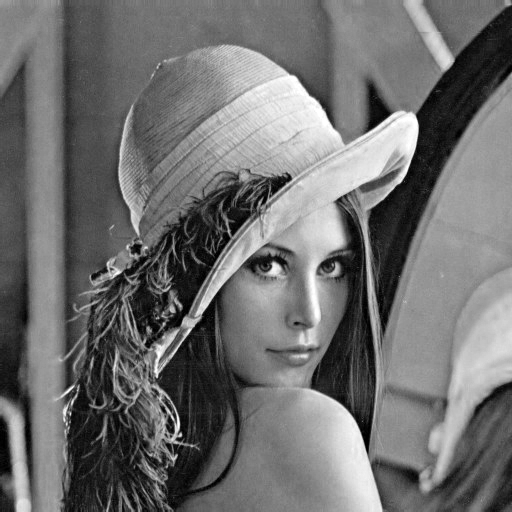
\includegraphics[width=0.21\linewidth]{img/Lena4}
	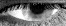
\includegraphics[width=0.21\linewidth]{img/Auge_4Gray}
	\caption{Ergebnis der Umwandlung von Farb- nach Grauwert mittels Extremwert-Verfahren. Oben: Max-Verfahren, Unten: Min-Verfahren}
	\label{img_MinMax}
\end{figure}
\begin{figure}
	\centering
	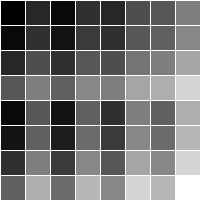
\includegraphics[width=0.21\linewidth]{img/Farbkarte3}
	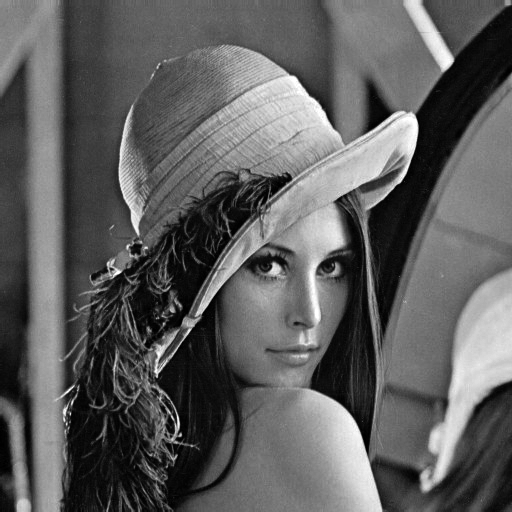
\includegraphics[width=0.21\linewidth]{img/Lena3}
	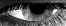
\includegraphics[width=0.21\linewidth]{img/Auge_3Gray}
	\caption{Ergebnis der Umwandlung von Farb- nach Grauwert mittels Quadrat-Verfahren}
	\label{img_Quadrat}
\end{figure}